
\section{Experimental data}
\label{sec:expdata}

In this section we summarize the data sets that have been used
in the present determination of the parton distribution of lead nuclei.
%
We also discuss the kinematical cuts and the  treatment of experimental
uncertainties.
%
Then we present the basic strategy that we adopt in this work
for the conversion of the
experimental data for the ratio of structure functions of different nuclei, $F_2^{A_1}$ and $F_2^{A_2}$, into
a common observable which is chosen to be the ratio of lead $F_2^{Pb}$ and deuteron $F_2^d$ structure
functions.


\subsection{Nuclear DIS structure functions data}


%
In this first study of nuclear PDFs with the NNPDF methodology
we restrict ourselves to fixed-target neutral current lepton-nuclei
deep-inelastic scattering structure functions.
%
In particular, we include the the
NMC~\cite{Amaudruz:1995tq,Arneodo:1995cs,Arneodo:1996rv,Arneodo:1996ru}, SLAC139~\cite{PhysRevD.49.4348} and EMC~\cite{Ashman:1992kv}
measurements of ratios of nuclear structure functions, defined
as
\be
\label{eqratio}
\frac{F_2^{A_1}(x,Q^2)}{F_2^{A_2}(x,Q^2)} \, .
\ee
The different types of nuclei $A_1$ and $A_2$ that are used in each
of these experiments is summarized in  Table~\ref{dataset}, as well
as the number of data points that survive our baseline kinematical
cuts and the corresponding publication reference.
%
In terms of neutral current DIS nuclear data, the experiments included
in Table~\ref{dataset} are the same of the EPS09 analysis.


%%%%%%%%%%%%%%%%%%%%%%%%%%
\begin{table}[t]
  \centering
  \small
\begin{tabular}{c c c c}
\hline
Experiment & $A_1/A_2$ & $N_{\rm dat}$ & Reference\\
\hline
\hline
  SLAC E-139 & He(4)/D & 2 & \cite{PhysRevD.49.4348} \\
  NMC 95, re. & He/D & 13 & \cite{Amaudruz:1995tq}\\
\hline
  NMC 95 & Li(6)/D & 12 & \cite{Arneodo:1995cs}\\
  NMC 95, $Q^2$ dependence & Li/D & 113 &\cite{Arneodo:1995cs}\\
\hline
  SLAC E-139 & Be(9)/D & 2 & \cite{PhysRevD.49.4348}\\
  NMC 96 & Be/C & 15 & \cite{Arneodo:1996rv}\\
\hline
  CERN EMC & C(12)/D & 9 & \cite{Ashman:1992kv}\\
  SLAC E-139 & C/D & 1 & \cite{PhysRevD.49.4348}\\
  NMC 95, NMC 95, re.  & C/D & 13 & \cite{Arneodo:1995cs,Amaudruz:1995tq}\\
  NMC 95, $Q^2$ dependence & C/D & 125 & \cite{Arneodo:1995cs}\\
  NMC 95, re. & C/Li & 10 & \cite{Amaudruz:1995tq}\\
\hline
  SLAC E-139 & Al(27)/D & 2 & \cite{PhysRevD.49.4348}\\
  NMC 96 & Al/C & 15 & \cite{Arneodo:1996rv}\\
\hline
  SLAC E-139 & Ca(40)/D & 1 & \cite{PhysRevD.49.4348}\\
  NMC 95, re. & Ca/D & 13 & \cite{Amaudruz:1995tq}\\
  NMC 95, re. & Ca/Li & 10 & \cite{Amaudruz:1995tq}\\
  NMC 96 & Ca/C & 15 & \cite{Arneodo:1996rv}\\
\hline
  SLAC E-139 & Fe(56)/D & 4 & \cite{PhysRevD.49.4348}\\
  NMC 96 & Fe/C & 15 & \cite{Arneodo:1996rv}\\
\hline
  CERN EMC & Cu(64)/D & 19 & \cite{Ashman:1992kv}\\
\hline
  SLAC E-139 & Ag(108)/D & 1 & \cite{PhysRevD.49.4348}\\
\hline
 CERN EMC & Sn(117)/C & 8 & \cite{Ashman:1992kv}\\
 NMC 96 & Sn/C & 15 & \cite{Arneodo:1996rv}\\
 NMC 96, $Q^2$ dependence  & Sn/C & 121 & \cite{Arneodo:1996ru}\\
\hline
  SLAC E-139 & Au(197)/D & 2 & \cite{PhysRevD.49.4348}\\
\hline
 NMC 96 & Pb/C & 15 & \cite{Arneodo:1996rv}\\
 \hline
 \hline
 Total & & 571 & \\
\hline
\end{tabular}
\caption{\small Data sets included in the present analysis.
  %
  In the second column we indicate the nuclei $A_1$ and $A_2$ which
  have been used in the measurement, see Eq.~(\ref{eqratio}),
  where when needed we indicate the atomic mass
  number in  parentheses.
  %
  In the third column the indicate the number of data points that
  survive the baseline kinematical cuts.
  %
  In the last column we indicate the corresponding publication reference.
}
\label{dataset}
\end{table}
%%%%%%%%%%%%%%%%%%%%%%%%%%%%%%%%%%%%%%


In this fit we use the standard kinematical cuts of the NNPDF unpolarized
fits, namely $Q^2 \ge Q^2_{\rm min}=3.5$ GeV$^2$ and $W^2 \ge W^2_{\rm min}=12.5$
GeV$^2$, which are chosen to minimize the impact of low scale non-perturbative
corrections and of higher twists.
%
Note that this cut is slightly more stringent that the
corresponding kinematical cut $Q^2 \ge 1.69$  used in
EPS09~\cite{Eskola:2009uj}.



Since the experimental covariance matrix is not available for any of
the nuclear DIS experiments summarized in Table~\ref{dataset},
we add in quadrature the statistical and systematic errors for each
data point, assuming that the systematic errors are fully uncorrelated
\be
\label{experr}
\sigma_i^{\rm exp,tot} = \lp \sigma_i^{\rm exp,stat}+\sigma_i^{\rm exp,sys}\rp^2 \, .
\ee
Note that since measurements are performed in terms of ratios of
structure functions between different nuclei, Eq.~(\ref{eqratio}),
common multiplicative systematic uncertainties such as luminosity will
cancel in the ratio.
%
As we discuss in the next section, we will add to
Eq.~(\ref{experr}) another contribution due to the theoretical
uncertainty in the conversion from Eq.~(\ref{eqratio}) to the ratio
of lead over deuteron structure functions
\be
\label{eqratio2}
\frac{F_2^{Pb}(x,Q^2)}{F_2^{d}(x,Q^2)} \, ,
\ee
which is the quantity which will be used for the nuclear
PDF fits presented in this work.

In Fig.~\ref{figkinplot} we show the
kinematical coverage in the $(x,Q^2)$ plane
  of the DIS nuclear data included in the present analysis,
  and summarized in Table~\ref{dataset}.
  %
  Only those points that satisfy the baseline kinematical
  cuts $Q^2 \ge Q^2_{\rm min}=3.5$ GeV$^2$ and $W^2 \ge W^2_{\rm min}=12.5$
GeV$^2$ are shown in this figure.

%%%%%%%%%%%%%%%%%%%%
\begin{figure}[t]
\begin{center}
  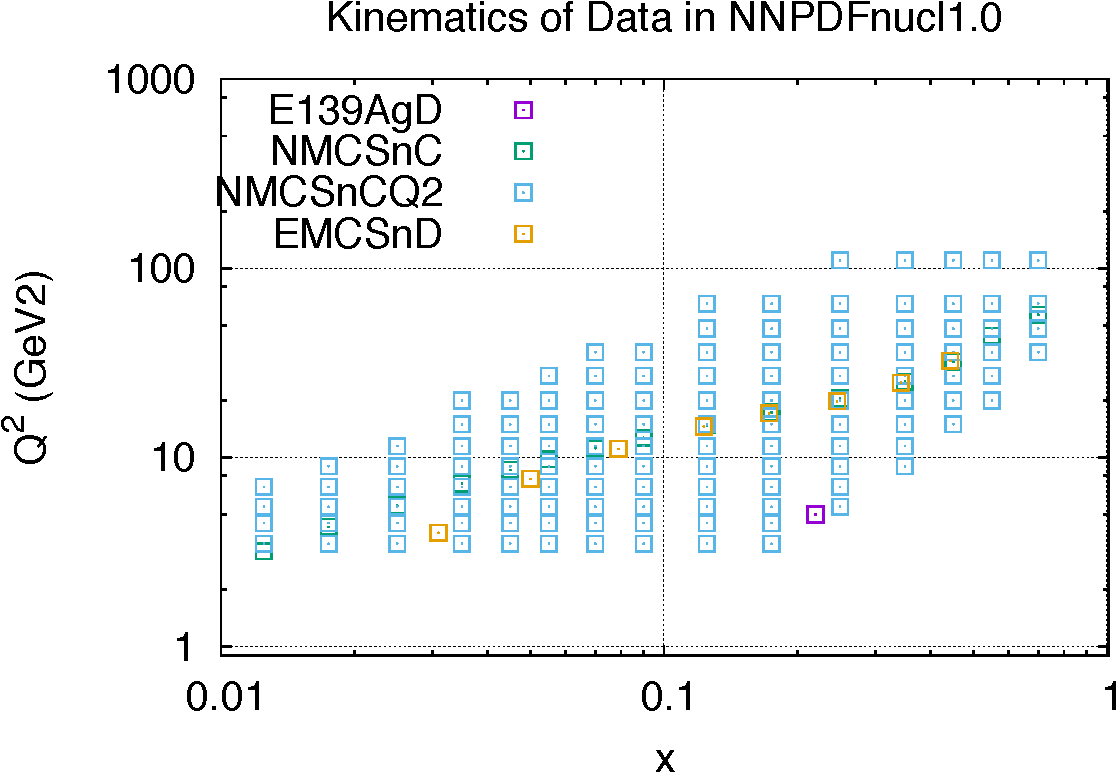
\includegraphics[width=0.70\textwidth]{plots/kinplot.pdf}
 \end{center}
\vspace{-0.3cm}
\caption{\small Kinematical coverage in the $(x,Q^2)$ plane
  of the DIS nuclear data included in the present analysis,
  and summarized in Table~\ref{dataset}.
  %
  Only those points that satisfy the baseline kinematical
  cuts $Q^2 \ge Q^2_{\rm min}=3.5$ GeV$^2$ and $W^2 \ge W^2_{\rm min}=12.5$
GeV$^2$ are shown in this figure.
}
\label{figkinplot}
\end{figure}
%%%%%%%%%%%%%%%%%%%%%%%



\subsection{Conversion of nuclear data to lead structure functions}
\label{sec:conversion}

In this section we explain the strategy that we use in this work based on the conversion of
experimental data for the ratio of structure functions of different nuclei, $F_2^{A_1}$ and $F_2^{A_2}$, into
a common observable which is chosen to be the ratio of lead $F_2^{Pb}$ and deuteron $F_2^d$ structure
functions.
%
The main advantage of this method is that it is not necessary anymore to determine from the data the
dependence of the nuclear modification ratios $R_{i}(x,Q^2,A)$ on the atomic mass number $A$.
%
Therefore, we can simply fit the parton distributions of nucleons in lead nuclei using exactly
the same technology as in the case of the unpolarized global NNPDF fits.
%
After presenting the  relevant conversion formulae,
we discuss how theoretical uncertainties are propagated from
the input nuclear PDFs used to the experimental data,
and show representative results for a variety of experiments.

The basic idea is the following.
%
Available nuclear DIS structure function data is presented as ratios
of structure functions measured on different nuclear targets
\be
\frac{F_2^{A_1}(x,Q^2)}{F_2^{A_2}(x,Q^2)} \, ,
\ee
and we would like to express these measurements in terms
of a common ratio of the lead structure functions over
the deuteron structure functions,
\be
\frac{F_2^{\rm Pb}(x,Q^2)}{F_2^{\rm d}(x,Q^2)} \, .
\ee
To achieve this, we use the results of a previous nuclear fit
to write this conversion as follows
\be
\label{eq:conversion2}
\lp  \frac{F_2^{\rm Pb}(x,Q^2)}{F_2^{\rm d}(x,Q^2)} \rp_{\rm exp+th}
= \lp \frac{F_2^{A_1}(x,Q^2)}{F_2^{A_2}(x,Q^2)} \rp_{\rm th}\cdot
\mathcal{C}_{\rm th}(x,Q^2, A_1,A_2) \ ,
\ee
where the theoretical conversion factor $\mathcal{C}_{\rm th}(x,Q^2, A_1,A_2)$
is evaluated using an existing nuclear PDF analysis as follows
\be
\label{eq:conversionfactor}
\mathcal{C}_{\rm th}(x,Q^2, A_1,A_2) \equiv
\lp \frac{F_2^{A_2}(x,Q^2)}{F_2^{A_1}(x,Q^2)} \rp_{\rm th} \cdot
\lp  \frac{F_2^{\rm Pb}(x,Q^2)}{F_2^{\rm d}(x,Q^2)} \rp_{\rm th} \ .
\ee

The  advantage of using the conversion factor
Eq.~(\ref{eq:conversionfactor}) is that a substantial fraction
of the nuclear PDF uncertainties (as well as many other theory
uncertainties such as higher perturbative orders) cancel
in the ratio of nuclear structure functions, specially
if $A_1$ is not to different to $A_2$.
%
Therefore, by ensuring that the theory uncertainty associated
to the conversion factor is not much larger than the experimental
uncertainty, we can reliably use the ratio
of lead to deuteron structure functions
Eq.~(\ref{eq:conversion2}) as a good proxy of the original
experimental measurements.
%
In addition, since the conversion factor is expressed
in terms of nuclear structure functions (which are fitted)
rather than in individual nuclear PDFs, we expect them
to be reasonably independent of the specific choice of
input nuclear PDF fit.



In the calculation of the conversion factor
Eq.~(\ref{eq:conversionfactor}) we use either the EPS09 or the
DSSZ NLO nuclear PDF fits.
%
For the free nucleon PDF we use the MSTW08 NLO set, consistently
with the original nuclear PDF fits, though we have checked
that the dependence on this choice is really mild due to
the cancellations in the ratios.
%
In the calculation of the structure function of deuterium
$F_2^{\rm d}$ we assume isospin symmetry and neglect
any nuclear effect, which are known to be negligible
as compared to the typical
uncertainties in nuclear PDF fits.\footnote{The impact
  of nuclear effects in unpolarized proton PDF analysis
  as been discussed for example in
  Refs.~\cite{Ball:2013gsa,Owens:2012bv,Harland-Lang:2014zoa}}.
%
The structure functions in Eq.~(\ref{eq:conversionfactor})
are computed using the original EPS09 fitting code, in a zero-mass
variable-flavor number scheme at NLO, and no target mass
corrections are included.
%
Note that the actual fit settings used to extract the
lead nuclear structure functions from Eq.~(\ref{eq:conversion2})
will be different, but the approximations enumerate
above are enough for the computation of the conversion factor.

The conversion factor Eq.~(\ref{eq:conversionfactor}) is affected
by the PDF uncertainties of the nuclear fit used in its computation.
%
In both EPS09 and DSSZ, PDF uncertainties are estimated with
the Hessian method~\cite{Pumplin:2001ct}.
%
Therefore, we can use the usual expressions for linear
error propagation in the Hessian approach to compute
the nuclear PDF uncertainties associated to
Eq.~(\ref{eq:conversionfactor}).
%
On the other hand, we neglect the free proton PDF uncertainties
from the MSTW08 set, which cancel to a very good approximation
in the ratios that define the conversion factor and that
are much smaller than nuclear PDF uncertainties.

In the Hessian approach, the PDF
uncertainties in a given cross-section
$\mathcal{O}=\mathcal{O}[f]$ can be computed as follows
\be
\left(\Delta \mathcal{O}\right)^2 = \frac{1}{4}\sum_{k=1}^{N_{\rm eig}}\left(\mathcal{O}[S_k^+]-\mathcal{O}[S_k^-]\right)^2,
\label{compression4}
\ee
where $\mathcal{O}[S_k^+]$ and $\mathcal{O}[S_k^-]$ denote the values of the quantity $\mathcal{O}$, computed by the nPDF error sets $S_k^+$ and $S_k^-$ and $S_0$ is the central PDF set, and $N_{\rm eig}$ is the number
of asymmetric eigenvectors of this Hessian PDF set.

Using Eq.~(\ref{compression4}), we can compute the nuclear
PDF uncertainty associated to the conversion factor as follows
\be
\left(\Delta \mathcal{C}\right)^2 = \frac{1}{4}\sum_{k=1}^{N_{\rm eig}}\left(\mathcal{C}[S_k^+]-\mathcal{C}[S_k^-]\right)^2 =
\frac{1}{4}\sum_{k=1}^{N_{\rm eig}}\left(
\frac{F_2^{A_2}(S_k^+)}{F_2^{A_1}(S_k^+)} 
 \frac{F_2^{\rm Pb}(S_k^+)}{F_2^{\rm d}(S_0)}
 -
\frac{F_2^{A_2}(S_k^-)}{F_2^{A_1}(S_k^-)} 
 \frac{F_2^{\rm Pb}(S_k^-)}{F_2^{\rm d}(S_0)}
 \right)^2 \, ,
\label{compression5}
\ee
where note that the deuteron structure functions are always
calculated with the central set $S_0$, since nuclear
PDF uncertainties are ignored in this case.
%
The correlation between the same eigenvector variations between
different nuclei ensures that the total
PDF uncertainty Eq.~(\ref{compression5}) associated to
the conversion factor will be typically rather smaller
than the corresponding experimental uncertainties, guaranteeing
the robustness of our strategy.

In Fig.~\ref{fig1aue139} we illustrate the typical size of
the PDF uncertainties associated with the conversion factor,
computed using Eq.~(\ref{compression5}), with the corresponding
experimental uncertainties for a number of representative datasets.
%
We show the results when the conversion factor is computed with
EPS09 and with DSSZ, as percentage compared to the central value
of the conversion factor.
%
As can be seen, for most of the points in $x$ and $Q^2$ the
PDFs uncertainties in the conversion factor are smaller than
the total experimental uncertainty.
%
Therefore, by cutting those data points for which the theory
error is too large, we can end up with a reduced nuclear
data set expressed in terms of $F_2^{\rm Pb}/F_2^{\rm d}$.

%%%%%%%%%%%%%%%%%%%%
\begin{figure}[t]
\begin{center}
  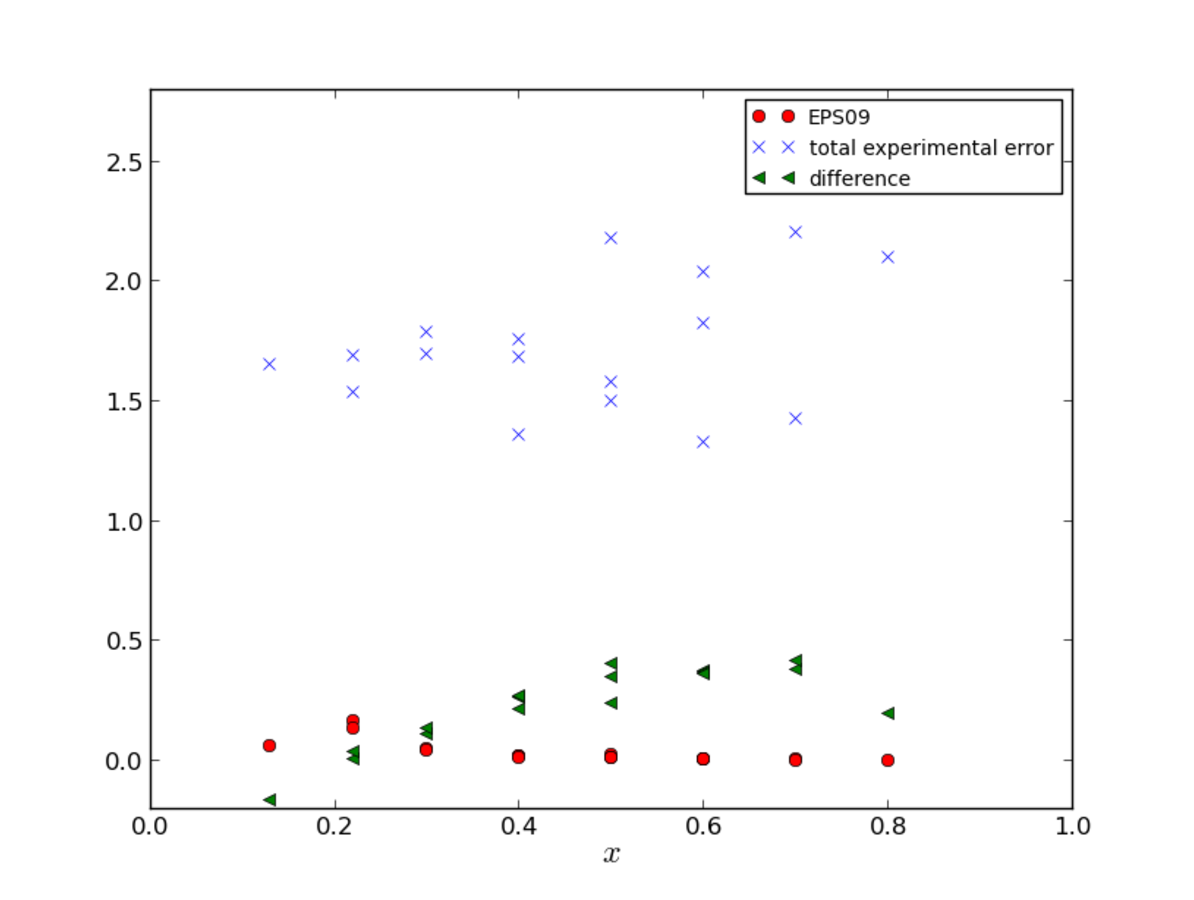
\includegraphics[width=0.49\textwidth]{plots/au_e139.pdf}
  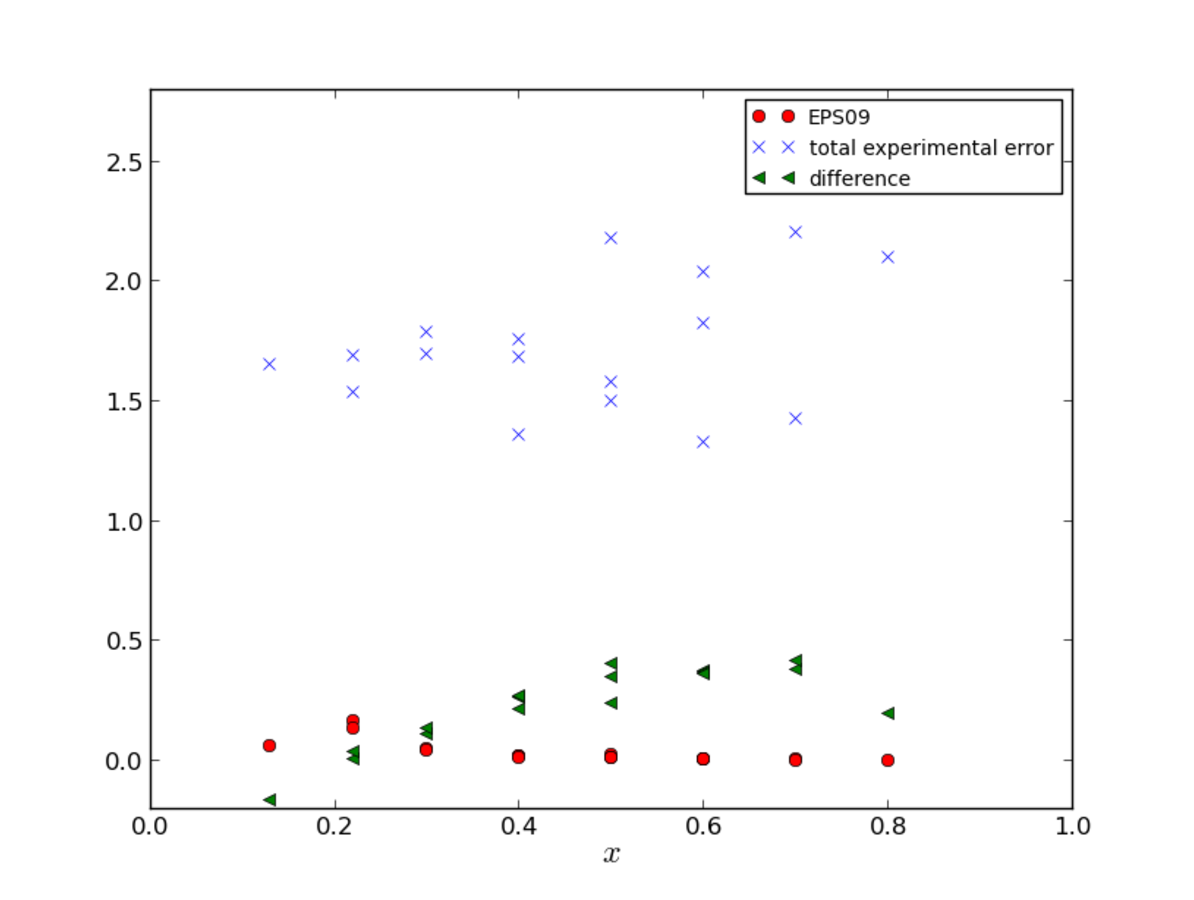
\includegraphics[width=0.49\textwidth]{plots/au_e139.pdf}
\end{center}
\vspace{-0.3cm}
\caption{\small Left plot: comparison of the magnitude
  of the total experimental uncertainty in
  percentage (blue crosses)
  with the size of the PDF uncertainty in the conversion
  factor, in percent computed with respect to the
  central value, using EPS09 as input PDF set, for
  the E139 experiment.
  %
  Right plot: the same comparison now using DSSZ as input
  in the calculation of the conversion factors.
}
\label{fig1aue139}
\end{figure}
%%%%%%%%%%%%%%%%%%%%%%%

Therefore, in this work we will keep only those data points
for the experiments listed in Table~\ref{dataset} which satisfy the
condition that
\be
\label{eq:condition}
\frac{\Delta \mathcal{C} }{\mathcal{C} } \le K_{\rm th} \cdot \frac{\sigma^{\rm exp,tot}}{
  \lp F_2^{A_1}/F_2^{A_1}\rp_{\rm exp}} \,  ,
\ee
where $\sigma^{\rm exp,tot}$ is the total experimental uncertainty,
Eq.~(\ref{experr}), and   $\lp F_2^{A_1}/F_2^{A_1}\rp_{\rm exp}$ is the
corresponding central value of the original experimental measurement.
%
The value of $K_{\rm th}$ cannot be much larger than 1, else our
nuclear PDF fit would be biased by the choice of input
nuclear PDF set.
%
In this work we will explore different choices for
$K_{\rm th}$ in the range $\lc 1.0,1.5\rc$, and study the stability
if the fit results with respect to this choice.

For the data points that satisfy the condition
Eq.~(\ref{eq:condition}) we add the theoretical uncertainty in
the conversion factor Eq.~(\ref{compression5})
as an additional systematic uncertainty.
%
This time however this new theory systematic is treated to be as fully
correlated among all the data bins of a given experiment,
since it is obtained from the same underlying set of
nuclear PDFs.
%
Therefore, the total experimental uncertainty taking into account the theoretical
uncertainty in the conversion factor will be
\be
\label{eq:total}
\sigma_i^{\rm exp,tot} = \lp \sigma_i^{\rm exp,stat,2}+\sigma_i^{\rm exp,sys,2}
+\sigma_i^{\rm th,2} \rp^{1/2} \, ,
\ee
where the theoretical error is defined as
\be
\sigma_i^{\rm th} \equiv  \frac{\Delta \mathcal{C} }{\mathcal{C} }
\cdot \lp  \frac{F_2^{\rm Pb}(x,Q^2)}{F_2^{\rm d}(x,Q^2)} \rp_{\rm exp+th}
\ee
and where note that the statistical and systematic
experimental uncertainties have also been corrected
with the same conversion factor as the central
experimental data.

In Fig.~\ref{fig1nmc} we show representative subset of the NMC data
  on ratios of nuclear structure functions, after the conversion
  to the common ratio $F_2^{\rm Pb}/F_2^{\rm d}$ using the strategy
  discussed in the text.
  %
  In the upper plots the conversion has been performed using EPS09,
  while in the lower plots it has been done using DSSZ.
  %
  In both cases, the corresponding theoretical uncertainty from
  the conversion factor has been added in quadrature to
  the total experimental uncertainty, as
  indicated in Eq.~(\ref{eq:total}).

%%%%%%%%%%%%%%%%%%%%
\begin{figure}[t]
\begin{center}
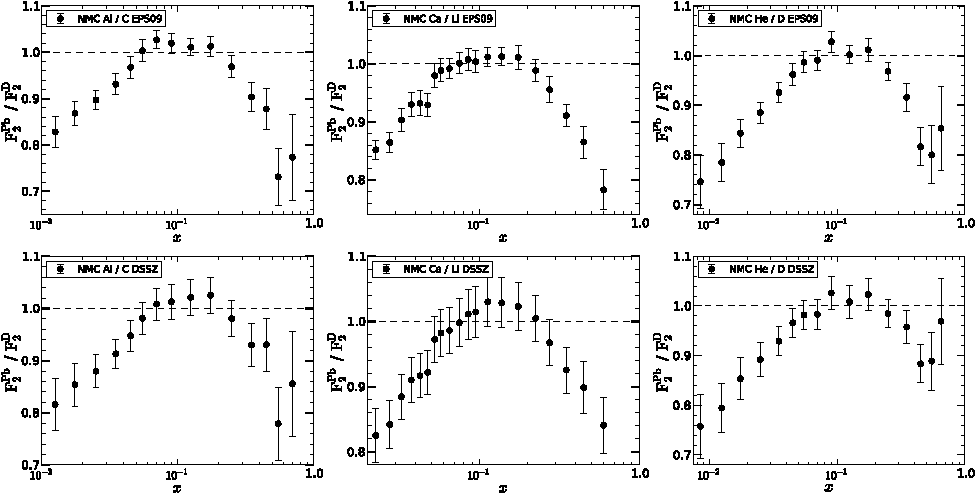
\includegraphics[width=0.98\textwidth]{plots/fig1nmc.pdf}
\end{center}
\vspace{-0.3cm}
\caption{\small A representative subset of the NMC data
  on ratios of nuclear structure functions, after the conversion
  to the common ratio $F_2^{\rm Pb}/F_2^{\rm d}$ using the strategy
  discussed in the text.
  %
  In the upper plots the conversion has been performed using EPS09,
  while in the lower plots it has been done using DSSZ.
  %
  In both cases, the corresponding theoretical uncertainty from
  the conversion factor has been added in quadrature to
  the total experimental uncertainty.
}
\label{fig1nmc}
\end{figure}
%%%%%%%%%%%%%%%%%%%%%%%

%%%%%%%%%%%%%%%%%%%%%%%%%%%%%%%%%%%%%%%%%%%%%%%%%%%%%%%%%%
